\documentclass{article}
\usepackage[nonatbib]{neurips_2019}
\usepackage[backend=bibtex, style=ieee]{biblatex}
\usepackage{graphicx}
\usepackage{hyperref}
\usepackage{siunitx}
\usepackage[table]{xcolor}


\bibliography{report}
\title{Human silhouette segmentation in videos}
\author{Miroslav Vitkov \\ sir.vorac@gmail.com}


\begin{document}
\maketitle


\begin{abstract}
Gait is a prominent biometric with similar importance to face recognition.
It is feasible in the presence of heavy noise like darkness or low quality cameras.
The input to the recogniser algorithm is usually a segmented and deshadowed human silhouette.
This report presents an implementation\footnote{https://github.com/MiroslavVitkov/silhouette} of the segmentation step.
We use Histogram of Oriented Gradients for dimensionality reduction and a Support Vector Machine for detection followed by approximate median filter for segmentation.
\end{abstract}


\section{Introduction}
\subsection{Gait}
The interdisciplinary field of human identification via gait is now 42 years old.
Initially, glowing markers were used\cite{begin} for 38\% recognition accuracy, compared to random chance of 16.7\%.

Further development split into model-free and model-based methods.
Model-free methods look at pixels, one notable work being the gait energy model\cite{energy}.
Model-based approaches use a strong prior, e.g. a pendulum model of legs\cite{pendulum}.

Modern methods are dominated by motion vector estimated approaches, such as \cite{pyramid}
A recent improvement to \cite{pyramid} demonstrates human recognition accuracy of 96\% using a fusion of a visible spectrum camera, a Microsoft Kinetic and a wearable accelerometer\cite{robust}.


\subsection{Silhouette}
One common preprocessing step is adaptively thresholded background subtraction \cite{vehicle}.
Pixels in consecutive frames are compared and if the difference is less that a threshold value, classified as background and thus not interesting.
The threshold is generated by an exponential filter.
The difference is computed by sum of absolute difference (SAD) \cite{background}.
This allows the procedure to ignore periodic noise e.g waving tree leaves and low-frequency noise e.g. parked car or change of illumination level.

The Histograms of Oriented Gradients (HOG)\cite{hog} descriptor encodes an an image's local colour gradients.
It works in a sliding window of square or circular shape.
Horizontal and vertical derivatives are calculated with a centered mask (1 0 1).
All generated values in the window are summarised into one tuple (direction, magnitude).
This approach is believed to work better than the earlier Local Binary Patterns.

\subsection{Cascade Classification}
Cascading is a type of ensemble learning.
It means connecting several weak classifiers in series and using all of the output data of one classifier as input to the next stage.
The pioneer was the Viola–Jones object detection framework, which we are using in this project.


\subsection{SVM}
Support Vector Machine is a classification algorithm, which draws a hyperplane in between training samples.
At test time, samples are classified based on their geometric position relative to the plane.


\subsection{HAAR-like features}
Consider adjacent rectangular regions at a specific window, sum up the pixel intensities inside each and form the difference.
The individual classifiers are weak (i.e. slightly better than random chance).
The key advantage of HAAR-like features is their constant-time estimation over an integral image representation.


\subsection{Histogram of Oriented Gradients descriptor}
The HOG image descriptor serves to encode image information in form of colour gradient direction and magnitude.
It is computed over a moving (multi-pixel) window, thus reduced the dimensionality.


\section{Dataset}
\subsection{What is out there}
Numerous human tracking outdoor datasets are described in the literature\cite{datasets0}\cite{datasets1}.
Notable is the occlusion dataset\cite{datasets2}, providing experience close to real world outdoor surveillance.
Also the AVA indoor dataset\cite{ava} consists of a large number (1200) single view videos.

\subsection{What was chosen}
The best silhouette segmentation dataset seems to be Supervisely's human dataset\cite{supervisely}. This is a sample from it:
\\
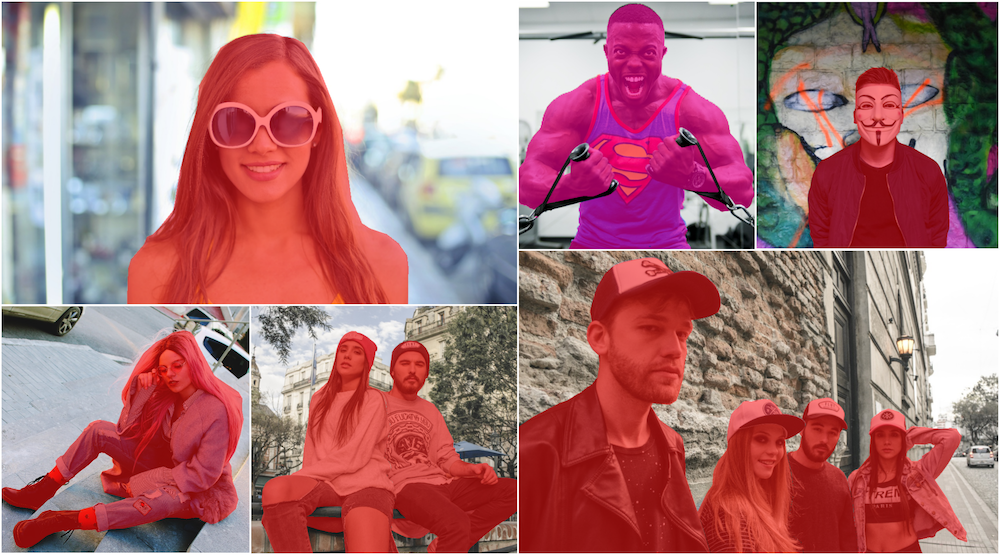
\includegraphics[height=0.5\textwidth]{../img/supervisely}
\\
compare it to COCO's segmented silhouettes:
\\
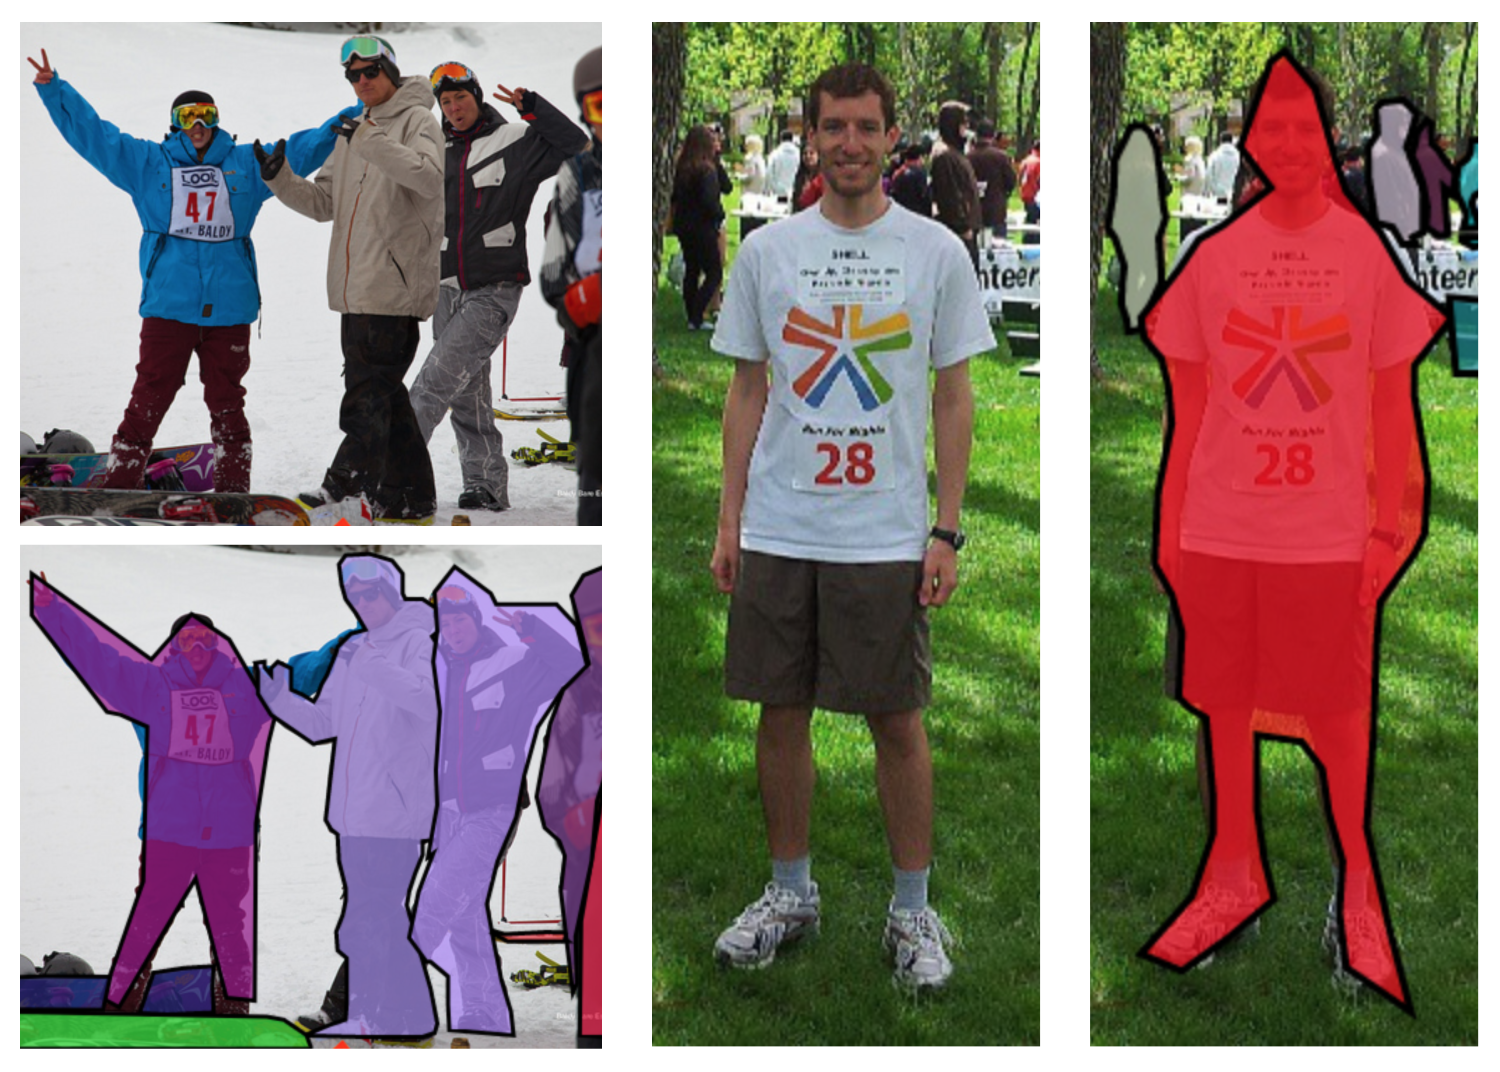
\includegraphics[height=0.5\textheight]{../img/coco}.

\subsection{In addition to that}
Segmenting silhouettes by static images isn't feasible.
To facilitate the task, a dataset of videos was compiled.
It is intended to facilitate frame-to-frame adaptive background subtraction in preselected regions to generate the actual silhouettes.
It consists of 1 video of a single walking subject, totalling 49 seconds of footage.


\section{Foreground/Background Segmentation}
A Gaussian Mixture model of the background is generated\cite{knn_background_subt}.
The model has a probability density function for each pixel separately.
A pixel is considered to be 'background' if it is well predicted by the density function.


\section{Video Captioning}
The detected silhouettes can be used for action detecion, velocity estimation, agent tracking.
Once again due to the poor performace of the pedestrai detector, no satisfiable tracking was performed, foiling further efforts.


\section{Method}
The RGB frame is scanned for pedestrians.
If any are detected, the foreground/background model is consulted at those locations.
It's output is the segmented silhouettes.


\section{Results}
\subsection{Measurement}
A true detection is one where the predicted bounding box covers a ground truth box more than 50\%.

% accuracy = tp / num predictions
% recall = tp / all actual positive
%total real: 1530, true_positives: 253, false positives: 1857 HOG accracy 253/1530, recall 253/1530
%total real: 1530, true_positives: 110, false positives: 682 LBP
\subsection{Detection}
On the Supervisely Human Dataset, the detection accuracy is 12.0\% and the recall is 16.5\% for the HOG+SVM setup.
The LBP performed at accuracy 12.8\%, recall 7.2\%.

Here we can see how artificial edges confuse the HOG descriptor.
\\
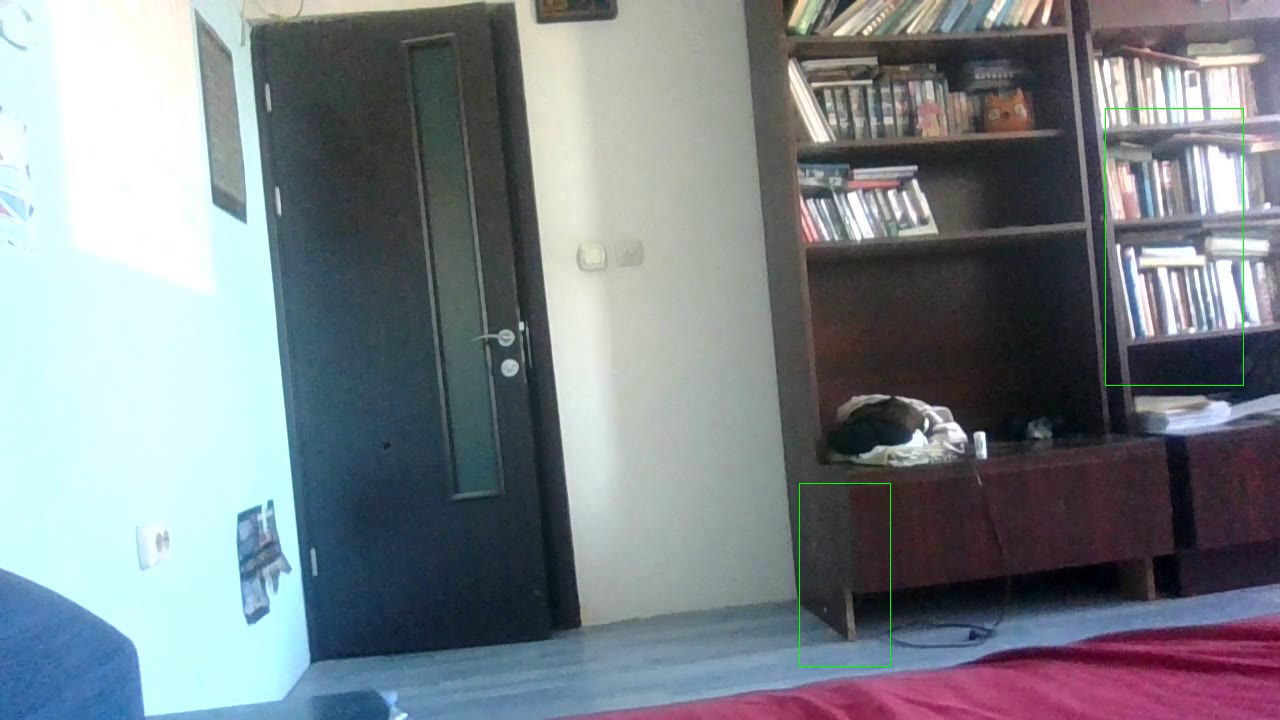
\includegraphics[height=0.5\textheight]{../img/false-positives}
\\
Even when a positive example is in clear view, no method achieved good results.
\\
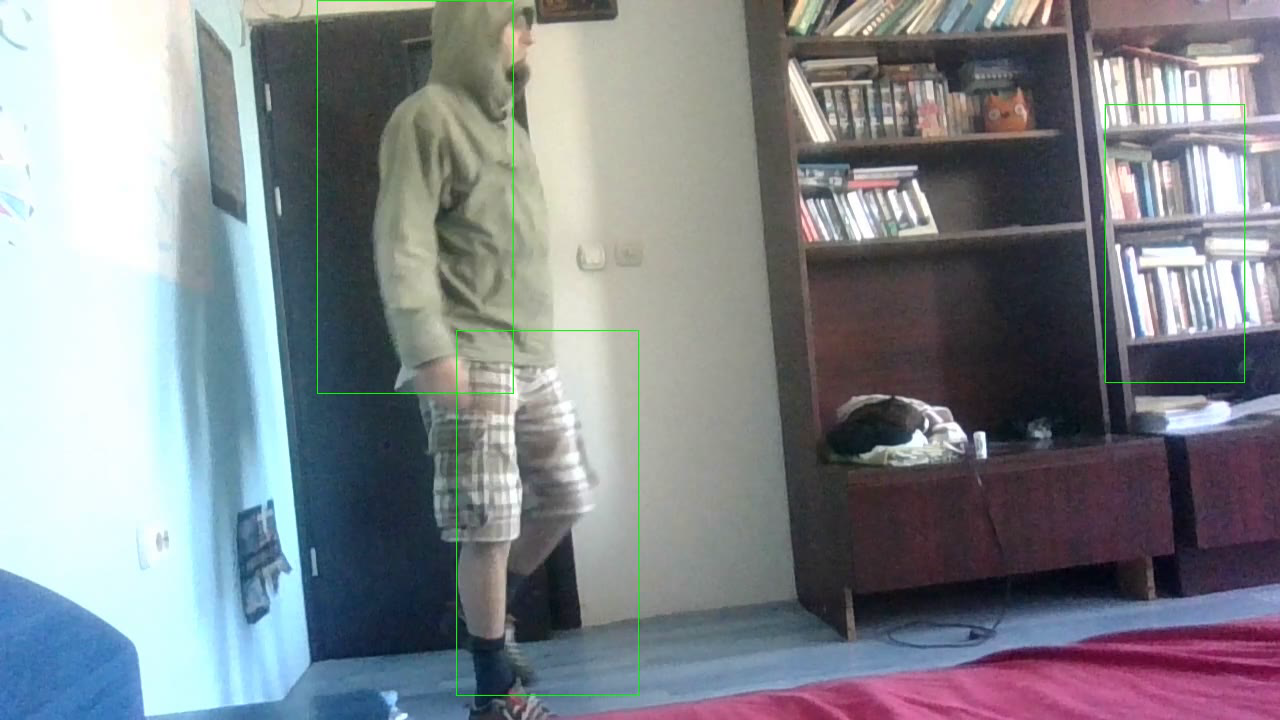
\includegraphics[height=0.5\textheight]{../img/pedestrian}
\\

\subsection{Segmentation}
The segmentation accuracy on the test video was close to 0\% due to inconsistent performance of the detector.
This can probably be mitigated by looking at the video as a whole and demanding smooth movement of pedestrians.


\section{Conclusion}
The effort was thwarted by the mediocre performance of the pedestrian detector.

One considered approach was tracking detected humans between frames.
It was not pursued because of the sheer amount of false positives.

A computational optimisation was conceived but not implemented: use the background detector to provide attention for the detector.


\printbibliography


\end{document}

